%\documentstyle[10pt,twoside]{article}
%\documentstyle[twoside]{article}
\documentclass[twoside]{article}
\setlength{\oddsidemargin}{0.25 in}
\setlength{\evensidemargin}{-0.25 in}
\setlength{\topmargin}{-0.6 in}
\setlength{\textwidth}{6.5 in}
\setlength{\textheight}{8.5 in}
\setlength{\headsep}{0.75 in}
\setlength{\parindent}{0 in}
\setlength{\parskip}{0.1 in}

\usepackage{graphicx}
\usepackage{url}

%
% The following commands sets up the lecnum (lecture number)
% counter and make various numbering schemes work relative
% to the lecture number.
%
\newcounter{lecnum}
\renewcommand{\thepage}{\thelecnum-\arabic{page}}
\renewcommand{\thesection}{\thelecnum.\arabic{section}}
\renewcommand{\theequation}{\thelecnum.\arabic{equation}}
\renewcommand{\thefigure}{\thelecnum.\arabic{figure}}
\renewcommand{\thetable}{\thelecnum.\arabic{table}}
\newcommand{\dnl}{\mbox{}\par}

%
% The following macro is used to generate the header.
%
\newcommand{\lecture}[4]{
   \pagestyle{myheadings}
   \thispagestyle{plain}
   \newpage
   \setcounter{lecnum}{#1}
   \setcounter{page}{1}
   \noindent
   \begin{center}
   \framebox{
      \vbox{\vspace{2mm}
    \hbox to 6.28in { {\bf CMPSCI~677~~~Distributed and Operating Systems
                        \hfill Spring 2018} }
       \vspace{4mm}
       \hbox to 6.28in { {\Large \hfill Lecture #1: #2  \hfill} }
       \vspace{2mm}
       \hbox to 6.28in { {\it Lecturer: #3 \hfill Scribe: #4} }
      \vspace{2mm}}
   }
   \end{center}
   \markboth{Lecture #1: #2}{Lecture #1: #2}
   \vspace*{4mm}
}

%
% Convention for citations is authors' initials followed by the year.
% For example, to cite a paper by Leighton and Maggs you would type
% \cite{LM89}, and to cite a paper by Strassen you would type \cite{S69}.
% (To avoid bibliography problems, for now we redefine the \cite command.)
%
\renewcommand{\cite}[1]{[#1]}

% \input{epsf}

%Use this command for a figure; it puts a figure in wherever you want it.
%usage: \fig{NUMBER}{FIGURE-SIZE}{CAPTION}{FILENAME}
\newcommand{\fig}[4]{
            %\vspace{0.2 in}
            \centerline{\includegraphics[scale=#2]{#4}}
            \begin{center}
            Figure \thelecnum.#1:~#3
            \end{center}
    }

% Use these for theorems, lemmas, proofs, etc.
\newtheorem{theorem}{Theorem}[lecnum]
\newtheorem{lemma}[theorem]{Lemma}
\newtheorem{proposition}[theorem]{Proposition}
\newtheorem{claim}[theorem]{Claim}
\newtheorem{corollary}[theorem]{Corollary}
\newtheorem{definition}[theorem]{Definition}
\newenvironment{proof}{{\bf Proof:}}{\hfill\rule{2mm}{2mm}}

% Some useful equation alignment commands, borrowed from TeX
\makeatletter
\def\eqalign#1{\,\vcenter{\openup\jot\m@th
  \ialign{\strut\hfil$\displaystyle{##}$&$\displaystyle{{}##}$\hfil
      \crcr#1\crcr}}\,}
\def\eqalignno#1{\displ@y \tabskip\@centering
  \halign to\displaywidth{\hfil$\displaystyle{##}$\tabskip\z@skip
    &$\displaystyle{{}##}$\hfil\tabskip\@centering
    &\llap{$##$}\tabskip\z@skip\crcr
    #1\crcr}}
\def\leqalignno#1{\displ@y \tabskip\@centering
  \halign to\displaywidth{\hfil$\displaystyle{##}$\tabskip\z@skip
    &$\displaystyle{{}##}$\hfil\tabskip\@centering
    &\kern-\displaywidth\rlap{$##$}\tabskip\displaywidth\crcr
    #1\crcr}}
\makeatother

% **** IF YOU WANT TO DEFINE ADDITIONAL MACROS FOR YOURSELF, PUT THEM HERE:



% Some general latex examples and examples making use of the
% macros follow.

\begin{document}

%FILL IN THE RIGHT INFO.
%\lecture{**LECTURE-NUMBER**}{**DATE**}{**LECTURER**}{**SCRIBE**}
\lecture{10}{Feb 28}{Prashant Shenoy}{\textbf{Utkarsh Srivastava}}

\section{Message Oriented Communication}
The communication can be classified along 2 dimensions: whether the system is persistent or transient; and whether it is synchronous or asynchronous.

\begin{description}
  \item[Persistence] : With persistent communication, messages are stored at each intermediate hop along the way until the next node is ready to take delivery of the message. It is also called a store and forward based delivery paradigm. A good example is the postal system (pony express), email, etc. 
  
  For transient communication, messages are buffered only for small periods of time (as long as sending/receiving applications are executing). If the message cannot be delivered or the next host is down, it is discarded. Example: General TCP/IP communication.
  
  \item[Synchronicity] : With synchronous communication. the sender blocks further operation until some sort of an acknowledge or response is received, hence the name blocking communication.
  
  With asynchronous communication or non-blocking communication, the sender continues execution without waiting for any acknowledgement or response. Hence, need a local buffer at the sender to deal with it at a later stage. 
\end{description}

\section{Combinations - Persistence and Synchronicity}

\begin{figure}
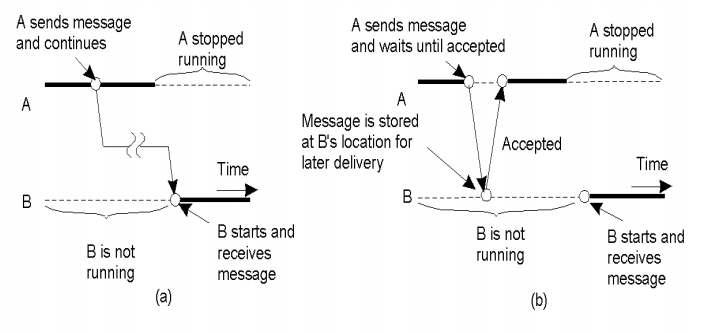
\includegraphics[width=15cm, height=6cm]{Selection_001}
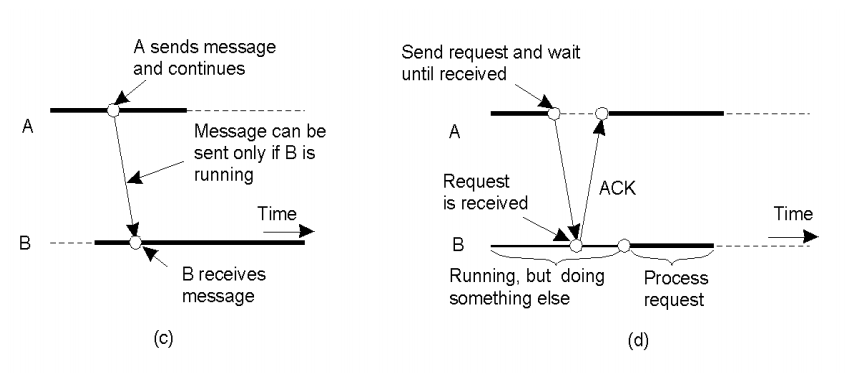
\includegraphics[width=15cm, height=6cm]{Selection_002}
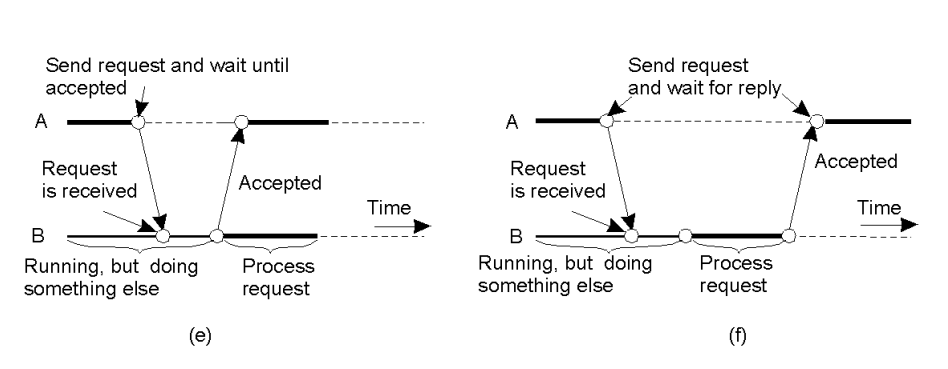
\includegraphics[width=15cm, height=6cm]{Selection_003}
\centering
\caption{Types of message-oriented communication (even though it seems as if 4 such combinations are possible, it can be further expanded to 6 such combinations based on the type of synchronisation acknowledgement): (a) Persistent + Asynchronous (b) Persistent + Synchronous (c) Transient + Asynchronous (d) Receipt-based Transient Synchronous (e) Delivery-based Transient Synchronous (f) Response-based Transient Synchronous}
\end{figure}

\subsection{Persistent Asynchronous}
Figure 10.1 (a) gives us a time-line map for persistent asynchronous communication. A is the sender and B is the receiver. Dark line depicts execution. A sends a message and keeps executing without blocking. The message sent from A will take an arbitrary amount of time to reach B. A may or may not be running by the time the message reaches B. For the same, disk or multiple memory queues could be used for storage at B's side. However, we get a guarantee that the message will eventually reach B. B receives this request and processes it then. Example: emails can take an arbitrary amount of time to reach, and when the receiver reads the email, the sender might not even be running. 

\subsection{Persistent Synchronous}
Figure 10.1 (b) explains persistent synchronous communication. Here, A sends a message, and then is blocked (depicted by the dotted line). The acknowledgement is for receipt (not delivery/response). Because this model is persistent, the message may stay in B's queue (or in any router along the way) for an arbitrary amount of time. Messaging or chat apps falls into this category. Many messaging systems are persistent, and can tell us the delivery status.

\subsection{Transient Asynchronous}
Figure 10.1 (c) explains this form of communication. A sends the message and continues execution (non-blocking). B has to be running, because if it is not running the message will be discarded. Even if any router along the way is down, the message will be discarded. UDP communication is an example of transient asynchronous communication. The function $MPI\_bsend$() is an implementation of this.


\subsection{Receipt-based Transient Synchronous}
Figure 10.1 (d) explains receipt-based transient synchronous communication. A's message to B is blocking (synchronous) until an ack is received. This ack simply tells us that the message was received at the other end. It does not tell us anything about whether the process has started.

% \begin{figure}[b]
% \centering
% \end{figure}

\subsection{Delivery-based Transient Synchronous}
Is an extension of receipt-based transient synchronous communication. As in figure 10.1 (e), A will resume running when B takes the delivery of the message. The ack comes a little bit later than the previous method. This is essentially asynchronous RPC because from the perspective of an RPC, we are not blocking for the reply.

\subsection{Response-based Transient Synchronous}
Figure 10.1 (f) explains this type of communication. A resumes execution upon receiving a response. That is, not only has the message been delivered, but it has been processed and the ack comes back in the form of a reply. This is traditional RPC. The client is blocked for the entire duration the reply comes back.

\textbf{QUESTION} : Is there a co-relation between the stopping/running of A \& B in `Persistent Synchronous' case?\\
\textbf{ANSWER} : NO 

\section{Message Oriented Transient Communication}
Berkeley Socket Primitives, and Message-Passing Interface (MPI) are examples of message-oriented transient communication. These systems do not use on-disk queues for message storing. Below, we map the MPI primitive functions to one of the above types. MPI\_bsend simply appends the outgoing message to the local send buffer, and then keeps running. Thus, it is transient asynchronous communication. MPI\_send sends a message and waits until copied to the remote buffer. This is similar to delivery-based transient synchronous communication. MPI\_ssend waits until receipt start and MPI\_sendrecv waits for a reply, classifying each to receipt based and reply based transient synchronous communication respectively. Hence, these constructs map very well to the 6 different communication types mentioned above.


\section{Message Oriented Persistent Communication}
This class of communication is called Message Queuing Systems (MQS). They use on-disk buffers to ensure persistence of messages over long periods of time. Commom open-source examples include RabbitMQ, ActiveMQ, ZeroMQ, etc. An application level example for this is emails. All emails are stored on disks til delivery. The queues have names/addresses which are used to explicitly put messages into the queue. Persistence neither guarantees the duration in which the message will be delivered, nor the reading of the message. It only ensures delivery. Thus, it is a loosely coupled communication. 

\begin{figure}
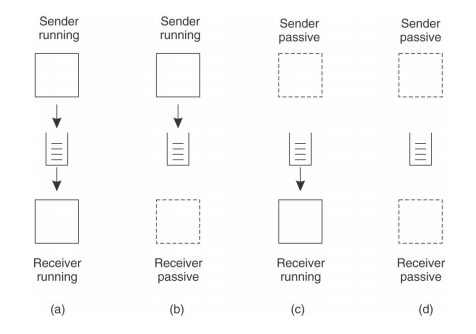
\includegraphics[width=15cm, height=6cm]{Selection_004}
\centering
\caption{Various use cases of a Message Queuing Model }
\end{figure}

Figure 10.2 explains the working of an MQS. The figure represents a series of queues as a single abstract persistent queue. Dark boxes indicate execution, while dotted boxes means the system is not running. The first case (a) is the simplest where both A and B are running, and the message is delivered immediately. In case (b) where B is not running, the message is stored at the queue and B takes delivery at a later point. In case (c), the sender is not running when B receives the message. In case (d), the message is queues for an arbitrary amount of time as both A and B are off. Thus, this is loose communication because the sender and the receiver are not participating in the communication at the same time.

The typical abstractions used in the message queing model are get() and put(). Put allows us to take a message and put it in a specific queue. Anyone who wants the delivery of the message will do a get() from the queue, followed by putting it in the next queue, or simply taking delivery (if it is the destination). Get and put are analogous to send and receive. We can have non-blocking poll as well, which will return the message if the queue is non-empty. Notify helps create a handler for notifications.

\textbf{QUESTION} : What if a scenario occurs when requests from 2 queues are posted simultaneously and one of those requests gets lost. How do we handle it?\\ 
\textbf{ANSWER} : Need a fail-case mechanism to be implemented internally if such a case ever arises.

\begin{figure}
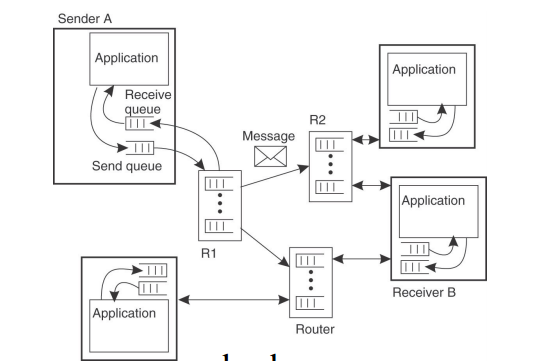
\includegraphics[width=12cm, height=6cm]{Selection_005}
\centering
\caption{General Architecture of an MQS}
\end{figure}

In a full-fledged MQS, we have MQS routers (with disk-queues) also called relays. Figure 10.3 shows an example of a typical MQS system. Message Brokers transform messages from one format to another, and are a part of many MQS'. This allows us to send messages across platforms, thus allowing interoperability. This is also used by many publish-subscribe systems, where a queue actually acts like a mailing list - having multiple receivers. The sender doesn't know who the message will be delivered to. 

IBM's Websphere MQ is a good example of MQS usage in a B2B system. It works with RPC along with API's for get/put etc. (like a pub-sub system). MicrosoftMQS is also an MQS, used for specific applications. These are fairly heavyweight, due to persistence. Example - ordering system. These are not typically used in web-based client-server architectures. The Message Channel Agent decides which router the message should be passed to next.

\textbf{QUESTION} : How does the broker perform its functionality when the message is encrypted?\\
\textbf{ANSWER} : If the encryption is end-to-end, then nothing much can be done. Otherwise, alternatives in terms of case-based operatability can be found.

\textbf{QUESTION} : Who knows about the routing information in such a set-up?\\
\textbf{ANSWER} : The rotuing protocol or at the app level, it is largely taken care of by the prefix table.

\textbf{QUESTION} : What functions does the Queue Manager perform?\\
\textbf{ANSWER} : (i) Looks at the routing table to gather information, (ii) Manages incoming to outgoing queue communication (which task to pick etc.)

\section{Stream Oriented Communication}
Stream oriented communication is usually used in audio and video streaming. Here, timeliness constraints become more important for quality streaming, especially for live video/audio. The data has to come in at a steady rate. Missing frame/audio packet will not be used if the player has already crossed that section of the video/audio. At times, the player may also freeze, waiting for the data to arrive. This is referred to as isochronous communication. In other words, data transfer from the server to the client imposes a delay (upper) bound. The problem is that internet is a best-effort network, and there are no guarantees on the delay. How can we still give good application performance when the underlying network does not provide any bounds on the delay? This is also coupled with the issue of network jitters - where in some time instance 100 packets could come in, whereas in some other 200 and in some as low as 20. This induces too much variability in the system. Another major difference from message oriented communication is that this is not a "client-pull" mechanism. The client only hits "play", and all the data is streamed to the player. This is the "server-push" model. This is emulated using HTTP (pull based) protocol.

There are 2 kinds: one where the file being streamed is stored on a disk, and other where we are streaming live from a (maybe multiple) camera/audio source. For the second type, the timeliness constraints are very stringent, as for the example of live video chat, we need the data to reach within the order of a hundred milliseconds. This includes the process of capture, encode and send. Another possibility is multi-cast - where the stream reaches multiple receivers. Typically, webcasts use this model (example - live stream of a sporting event). There is 1 transmission, and multiple receivers are tapped into the same live stream. 

\subsection{Quality of Service}
QoS is a way to encode the requirements of audio and video stream. The requirements include:
\begin{description}
\item[Bandwidth]: A HD video will need a minimum of a few Mbs per second.
\item[Maximum end-to-end delay bound]: Needs to be fixed to avoid playback glitches
\item[Jitter]: Refers to the variation in the end-to-end delay. The fluctuation in the delay is jitter. We want to minimize jitter to ensure a steady data rate.
\item[Loss]: Refers to the loss in data packets. With TCP, loss is handled using re-transmission. Fundamentally, in video streaming, retransmission may not be an option (especially for live transmissions). Late data might be as good as no data for live streaming. Time requirements can sometimes be a trigger for complex re-transmissions - hence we need to lower this.
\\
\textbf{QUESTION} : How does the client work to handle very long videos? \\
\textbf{ANSWER} : Either server-push model is implemented. Using client-pull model gets more complex but can be used with proper management of creating requests. Refer to the following diagram for that : 
\begin{figure}[h!]
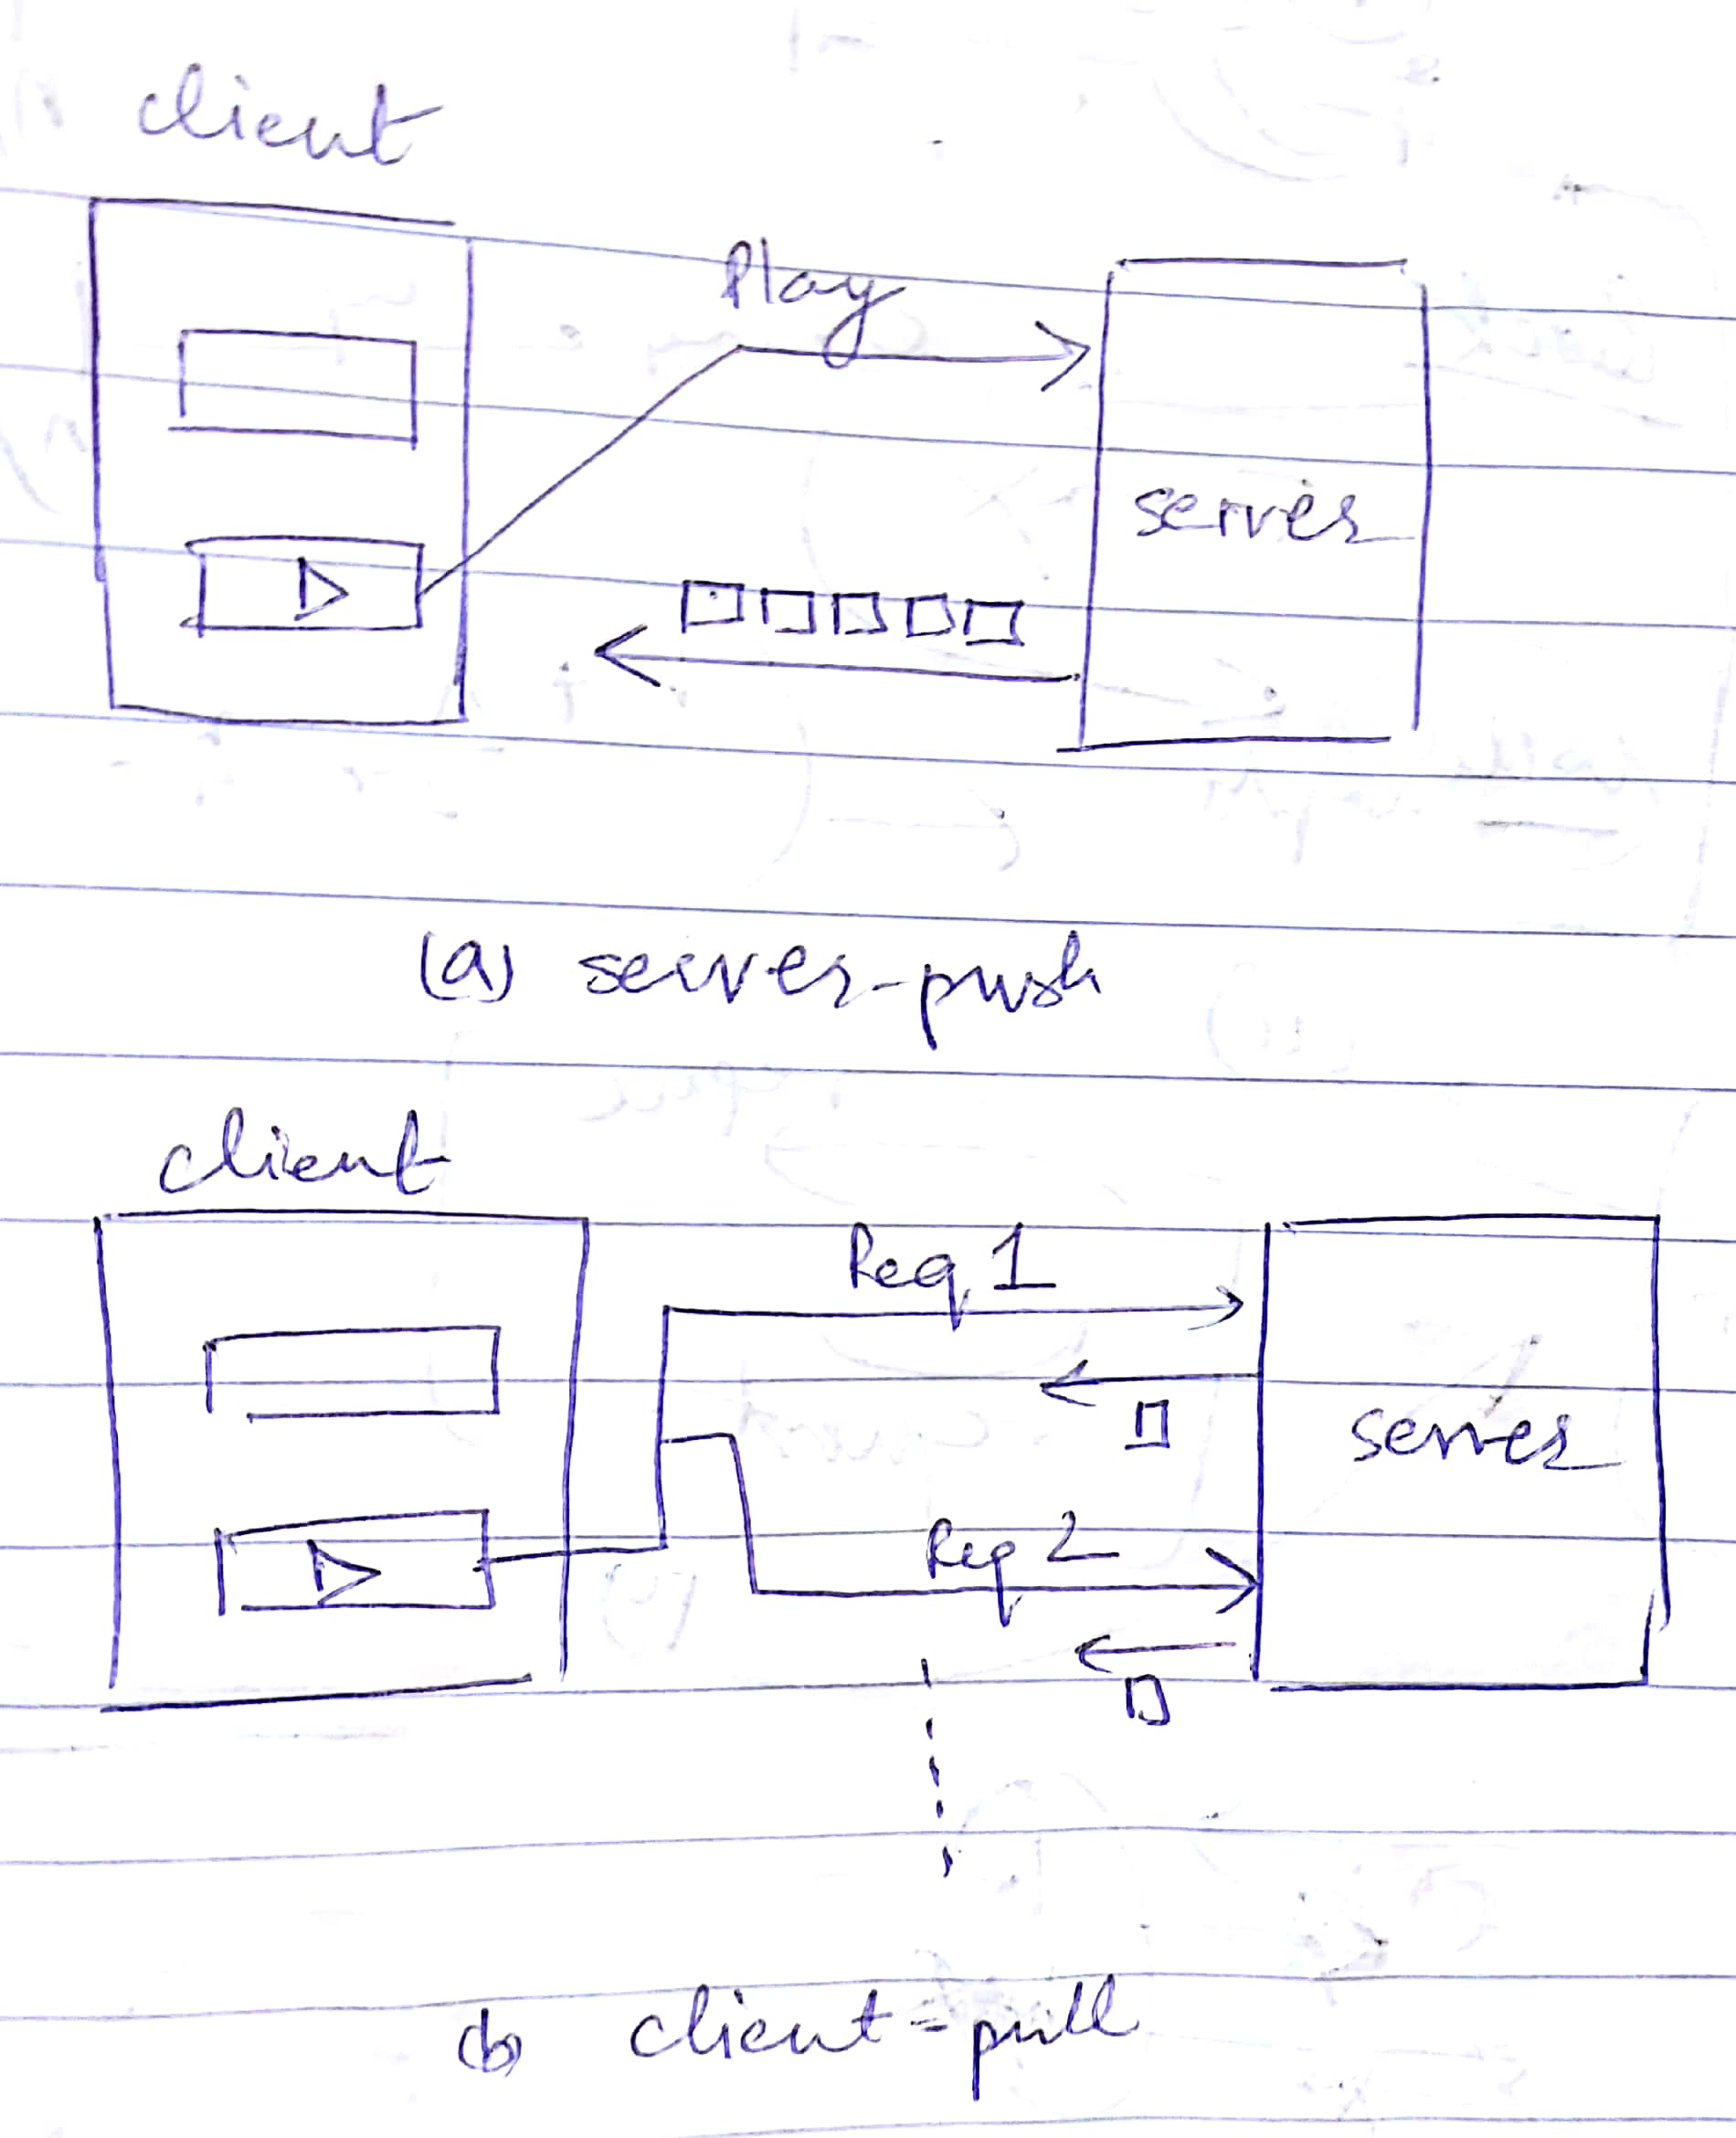
\includegraphics[scale=0.15]{Class_Diagram_1}
\centering
\caption{Architectures for handling playing of Long Videos}
\end{figure}


\end{description}
The network needs to support our requirements. However, explicit requirement support remained only in the research domain. Since the internet is a best-effort network, the only way in which we can enforce the above is by some degree of over-provisioning. There are no guarantees at all. A much more exhaustive list of QoS requirements is given in figure 10.4.

\begin{figure}[t]
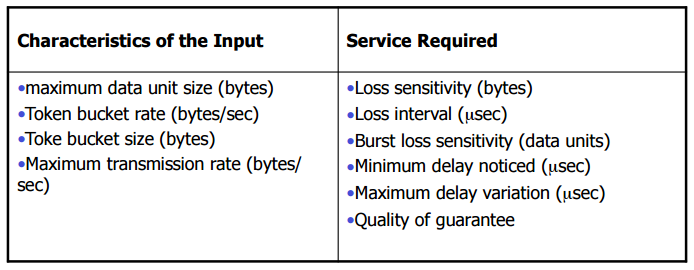
\includegraphics[scale=0.5]{Selection_006}
\centering
\caption{QoS Requirements}
\end{figure}


\subsection{Token Bucket}
Token Bucket is a OS-based method of enforcing QoS. Although it is not used in audio/video streaming, it is still used in many other contexts. It is also called a Leaky Bucket Rate Regulator. It enforces a certain bandwidth, using an OS-level mechanism. In general, it deals with the bandwidth bit-rate r and burst of deviation b.

Figure 10.5 explains the mechanism. Every time a packet needs to be sent, it needs to grab a token that will be generated by the OS. The OS will generate tokens at a steady rate R. R is the bandwidth that needs to be guaranteed. Thus, we can never send at a rate higher than the specified rate R because the packet will not be able to find any token. However, the token bucket allows for some instantaneous fluctuation, captured by the second parameter - depth of the bucket. Thus, the bucket has 2 parameters : token generation rate R and instantaneous depth B. When we start off, we start with a bucket of B tokens. That is, at any time, we can instantaneously generate B packets that can grab the B tokens and go out instantly. Then, the bucket will be filled at a steady rate of R. 

Essentially, the plot of the maximum number of packets sent vs time will give us a linear plot y=mx + b, where b=B and m=R, y is the number of packets sent and x is the time. This will mean that if we generate packets at a rate greater than R, they will have to wait, as the token corresponding to the packet will not have been generated. This also specifies the upper bound.


\begin{figure}[h!]
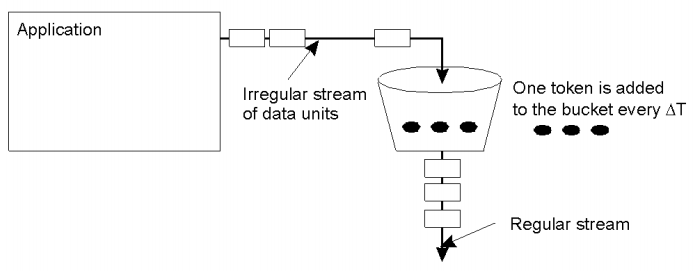
\includegraphics[scale=0.5]{Selection_007}
\centering
\caption{Leaky-Bucket model to ensure QoS}
\end{figure}

\begin{figure}[h!]
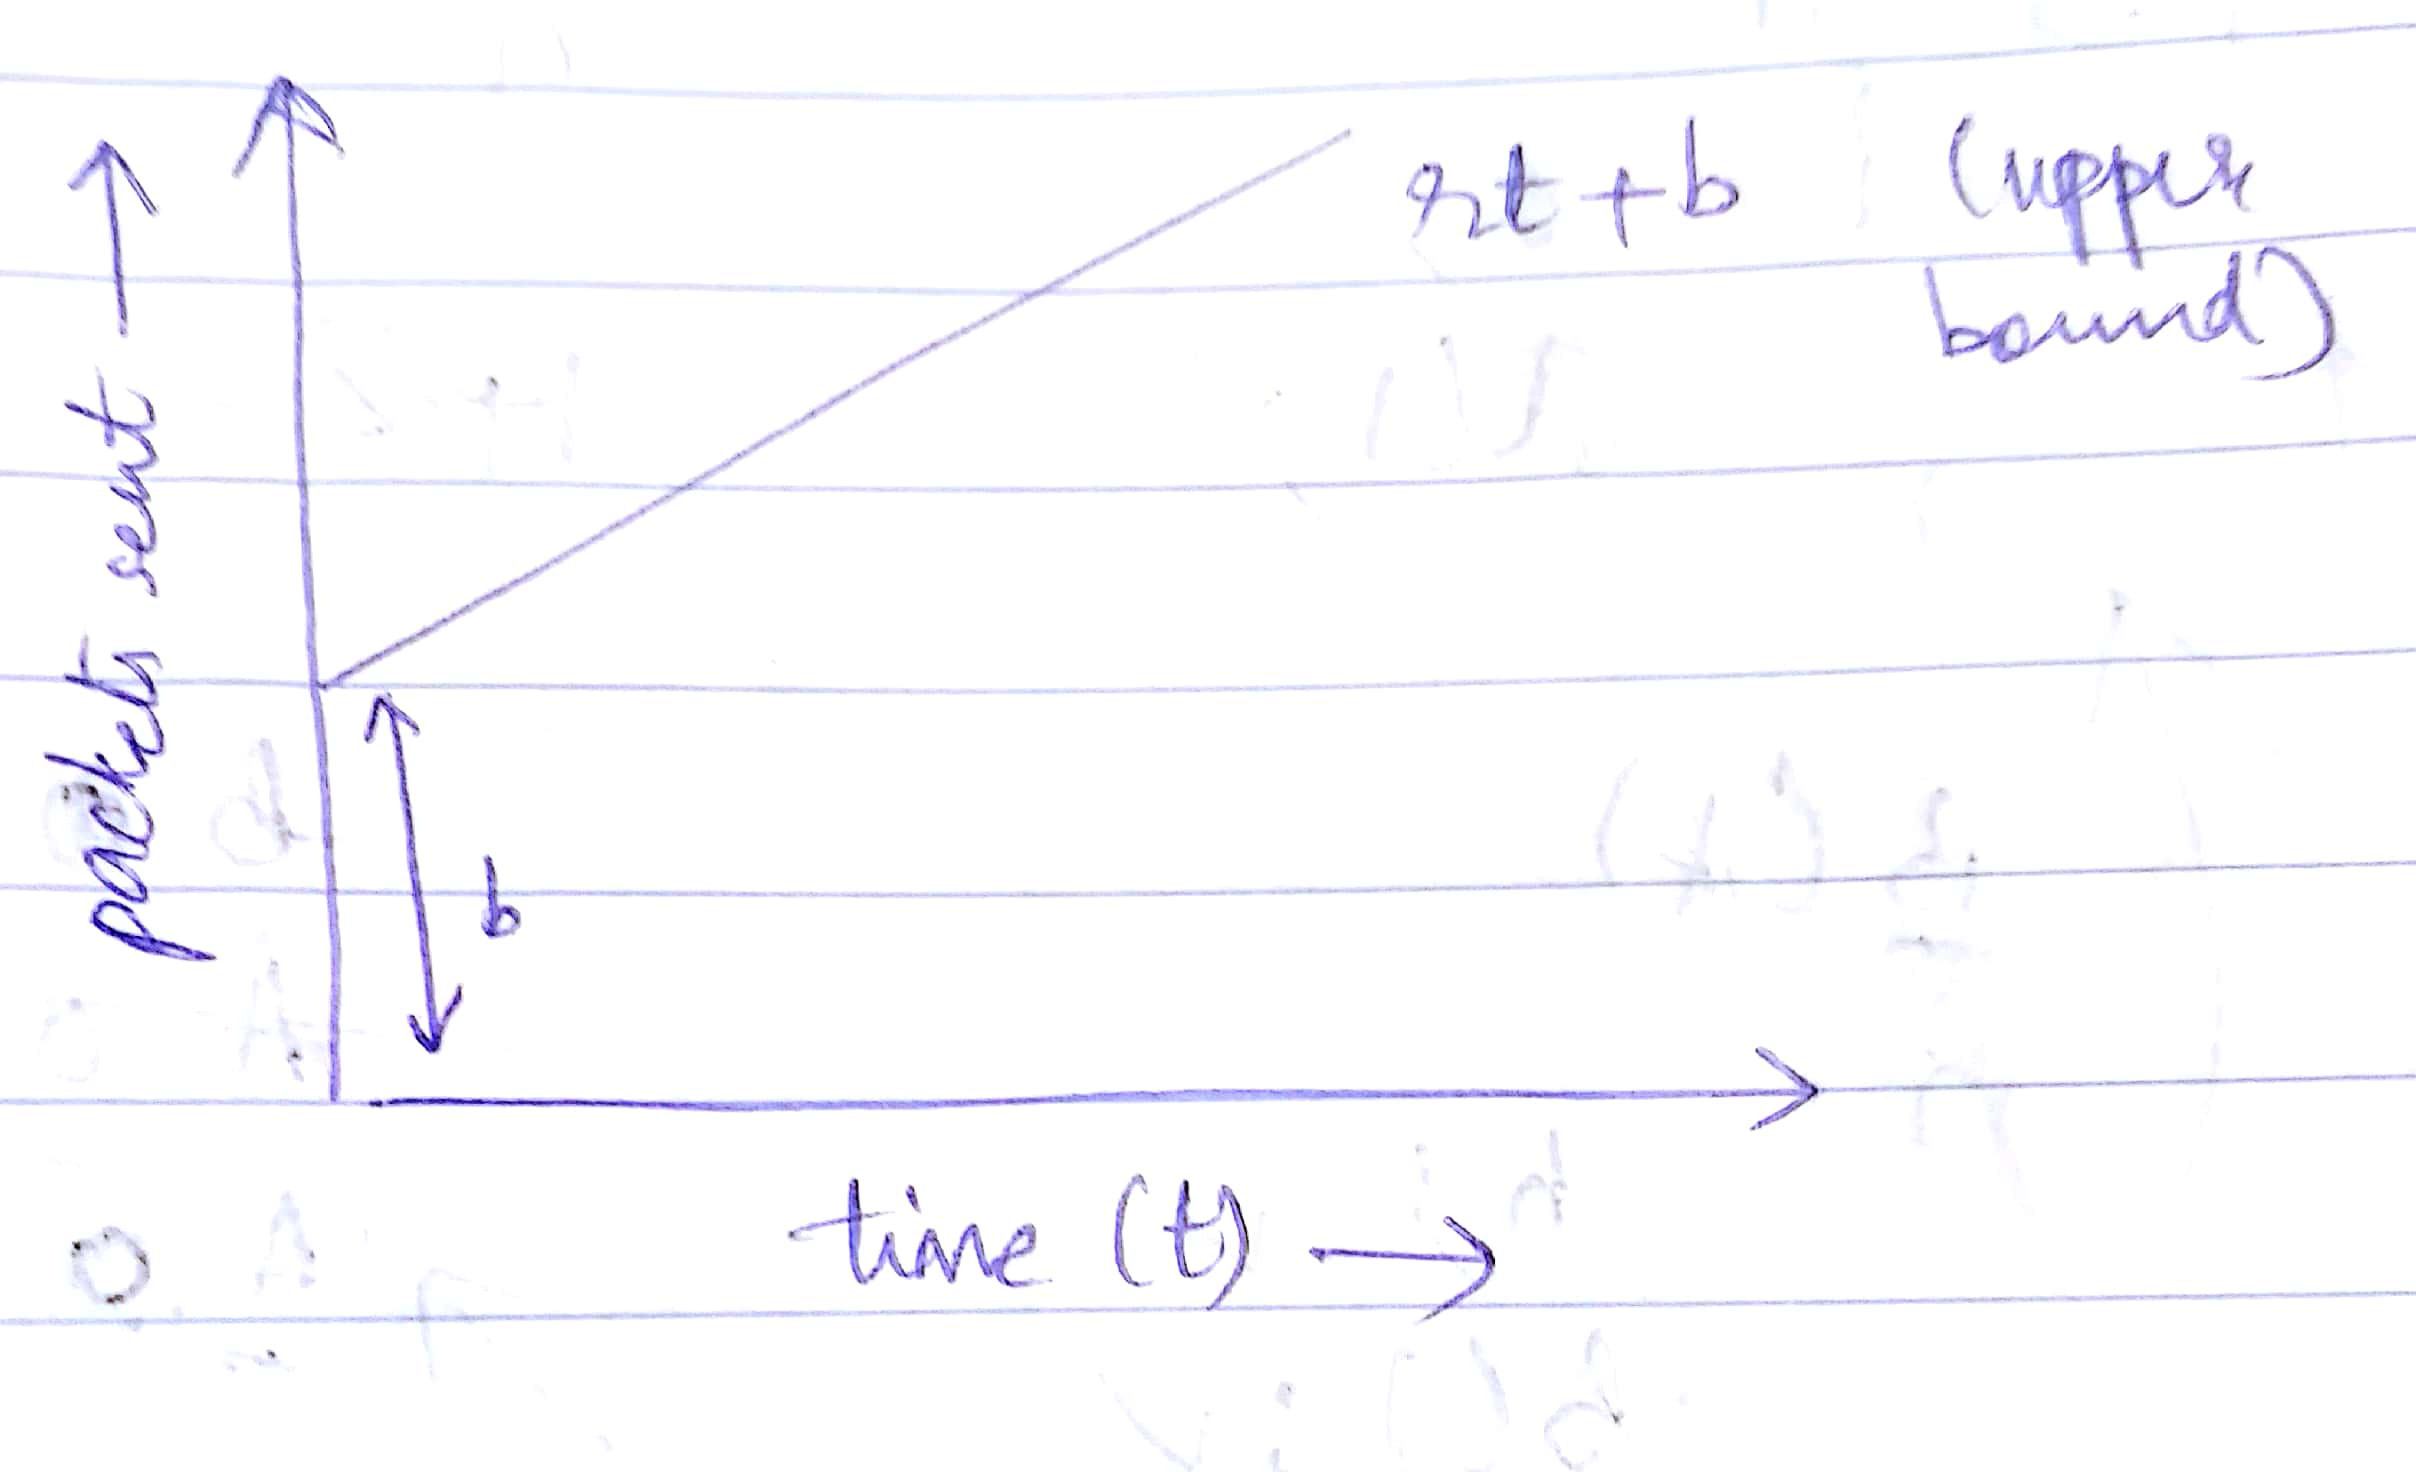
\includegraphics[scale=0.15]{Class_Diagram_2}
\centering
\caption{Packets Sent v/s Time (Token Bucket)}
\end{figure}


\textbf{QUESTION} : Why is `B' important? \\
\textbf{ANSWER} : Depending on the complexity of the event being streamed, it might require different compression and different rate of data transfers at different instances (e.g. in a football match, when showing players playing in the field v/s when showing the crowd)

\textbf{QUESTION} : What needs to be sent in such a system setting? \\
\textbf{ANSWER} : It is better to know the characteristics of data in such cases.

\textbf{QUESTION} : What is `R' dependent on? \\
\textbf{ANSWER} : It is an abstract concept and the requirements drive this selection.

\textbf{QUESTION} : Who sends out the token and how much? Is it done at the receiver?\\
\textbf{ANSWER} : It is done at the sender using defined policies based on the application needs.

\subsection{Using Buffers to Enforce QoS}
We want to reduce playback glitches in video streaming. First, we will handle delay. In Figure 10.6, the x axis is time, and each numbered box is a packet. These packets will have jitter because each will arrive at a different time, even though we sent them in steady gaps. To play at a constant fps (say f), we need to play the next frame in 1/f seconds. But, after frame 1 arrives, frame 2 does not arrive in that time difference, hence resulting in a playback glitch. We might be receiving at that rate on average, but there are no guarantees. One standard method is to hold the packets in a buffer before starting playback. Hopefully, if data continues to arrive at a good rate, our buffer will always have data, and we can keep playing. However, in the figure for example, frame 8 still arrives late resulting in a playback glitch.
\begin{figure}[t]
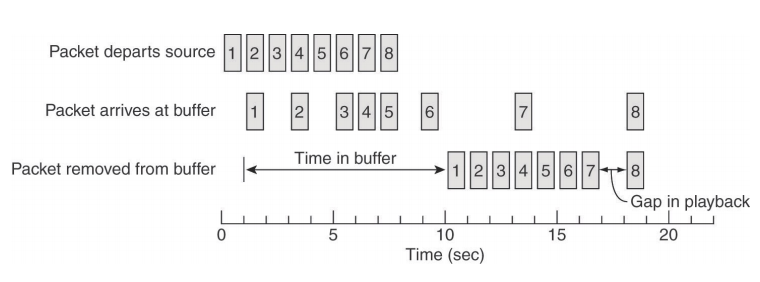
\includegraphics[scale=0.5]{Selection_008}
\centering
\caption{Handling playback glitches due to delays using buffers}
\end{figure}

One key question is how much should our buffer size be? The other issue is which packet to drop in the case of congestion to maintain loss information? The problem in dealing with packet loss needs to be handled, which is done using forward error correction (FEC) and scrambling of data packets, more of which will be covered in the next lecture.

\end{document}
